\chapter{场景建模与测试生成方法}
    \section{场景模型定义}
        \textbf{使用场景模型}是一种有效的模型化技术. 使用场景模型可以描述在现实世界中, 一或多个人如何与系统进行交互\footnote{http://agilemodeling.com/artifacts/usageScenario.htm}. 模型包括了交互过程中的步骤, 事件和动作. 本文提出了一种描述与web API的交互的使用场景模型. 为了基于模型进行测试生成, 模型着重于抽象以下web API的特点:
        
        \begin{itemize}
            \item 与使用场景相关的服务的元素. 这包括服务的功能, 请求数据, 响应数据, 执行约束等.
            
            \item 交互中, 各服务之间的交互. 这包括执行序列和序列内通信, 比如调用序列中之前某个服务的响应, 可能作为之后调用其他服务的参数.
            
            \item 不同交互操作的频率. 在有限测试资源的情况下, 对于测试资源的分配, 各个被测API需要有优先级顺序. 比如, 一些API可能在许多场景下都被用到, 被频繁地调用, 或者为许多其他API提供前置服务. 那么, 根据基于使用的测试原则, 这些频繁使用的API需要进行更多测试. 因此, 对API使用的分析与建模有助于优化对各个API和场景所生成的测试用例数量.
        \end{itemize}
        
        概率有限状态自动机(PFSA)可以有效描述相关服务, 执行序列和交互频率. 然而, 对于数据约束和服务通信, 它的能力有所不足. 我们的模型基于概率有限状态自动机进行扩展, 克服了这些不足.
        
        \subsection{背景: 概率有限状态自动机}
        
            概率有限状态自动机(PFSA)是非确定性有限状态自动机(NFA)的扩展. 它对非确定性有限状态自动机的转移, 起始状态和终止状态加入了概率因素. 对于每个串中读入的字符, 自动机会根据从当前状态出发的转移边的概率分布, 来从可选的转移边中选择一项进行转移. 状态的初始化和终止也具有类似的概率性质.
            
            根据Enrique Vidal等人的阐述\cite{enriquev05}, 一个基本的概率有限状态自动机具有如下的定义(定义\ref{def.pfsa}).
            
            \begin{definition}
                \label{def.pfsa}
                概率有限状态自动机为一个元组
                \begin{equation}
                    \mathcal{B} := <Q_{\mathcal{B}}, \Sigma, \sigma_{\mathcal{B}}, I_{\mathcal{B}}, F_{\mathcal{B}}, P_{\mathcal{B}}>,
                \end{equation}
                
                其中:
                \begin{itemize}
                    \item $Q_{\mathcal{B}}$是有限的状态集合;
                    \item $\Sigma$是字符集;
                    \item $\sigma_{\mathcal{B}} \subseteq Q_{\mathcal{B}} \times \Sigma \times Q_{\mathcal{B}}$是状态转移的集合;
                    \item $I_{\mathcal{B}} : Q_{\mathcal{B}} \to \mathbb{R}^{+}$是各个状态作为起始状态的概率分布;
                    \item $P_{\mathcal{B}} : \sigma_{\mathcal{B}} \to \mathbb{R}^{+}$是各个转移边的转移概率;
                    \item $F_{\mathcal{B}}: Q_{\mathcal{B}} \to \mathbb{R}^{+}$是于各个状态处终止的概率分布.
                \end{itemize}
                
                $I_{\mathcal{B}}$函数满足初始状态概率归一化性质:
                \begin{equation}
                    \sum_{q \in Q_{\mathcal{B}}} I_{\mathcal{B}}(q) = 1.
                \end{equation}
                
                $P_{\mathcal{B}}$和$F_{\mathcal{B}}$函数满足转移概率归一化性质:
                \begin{equation}
                    \forall q \in Q_{\mathcal{B}}, F_{\mathcal{B}}(q) + \sum_{a \in \Sigma, q' \in Q_{\mathcal{B}}} P_{\mathcal{B}}(q,a,q') = 1.
                \end{equation}
            \end{definition}
            
            按照惯例, 概率有限状态自动机使用带标签边的有向图表示. 图\ref{fig:PFSA_example}展示了一个概率有限状态自动机的例子. 其中, 图的节点表示自动机的状态, 图的带标签边表示自动机的概率转移边, 图的节点数字表示自动机状态的终止概率.
            
            \begin{figure}
                \centering
                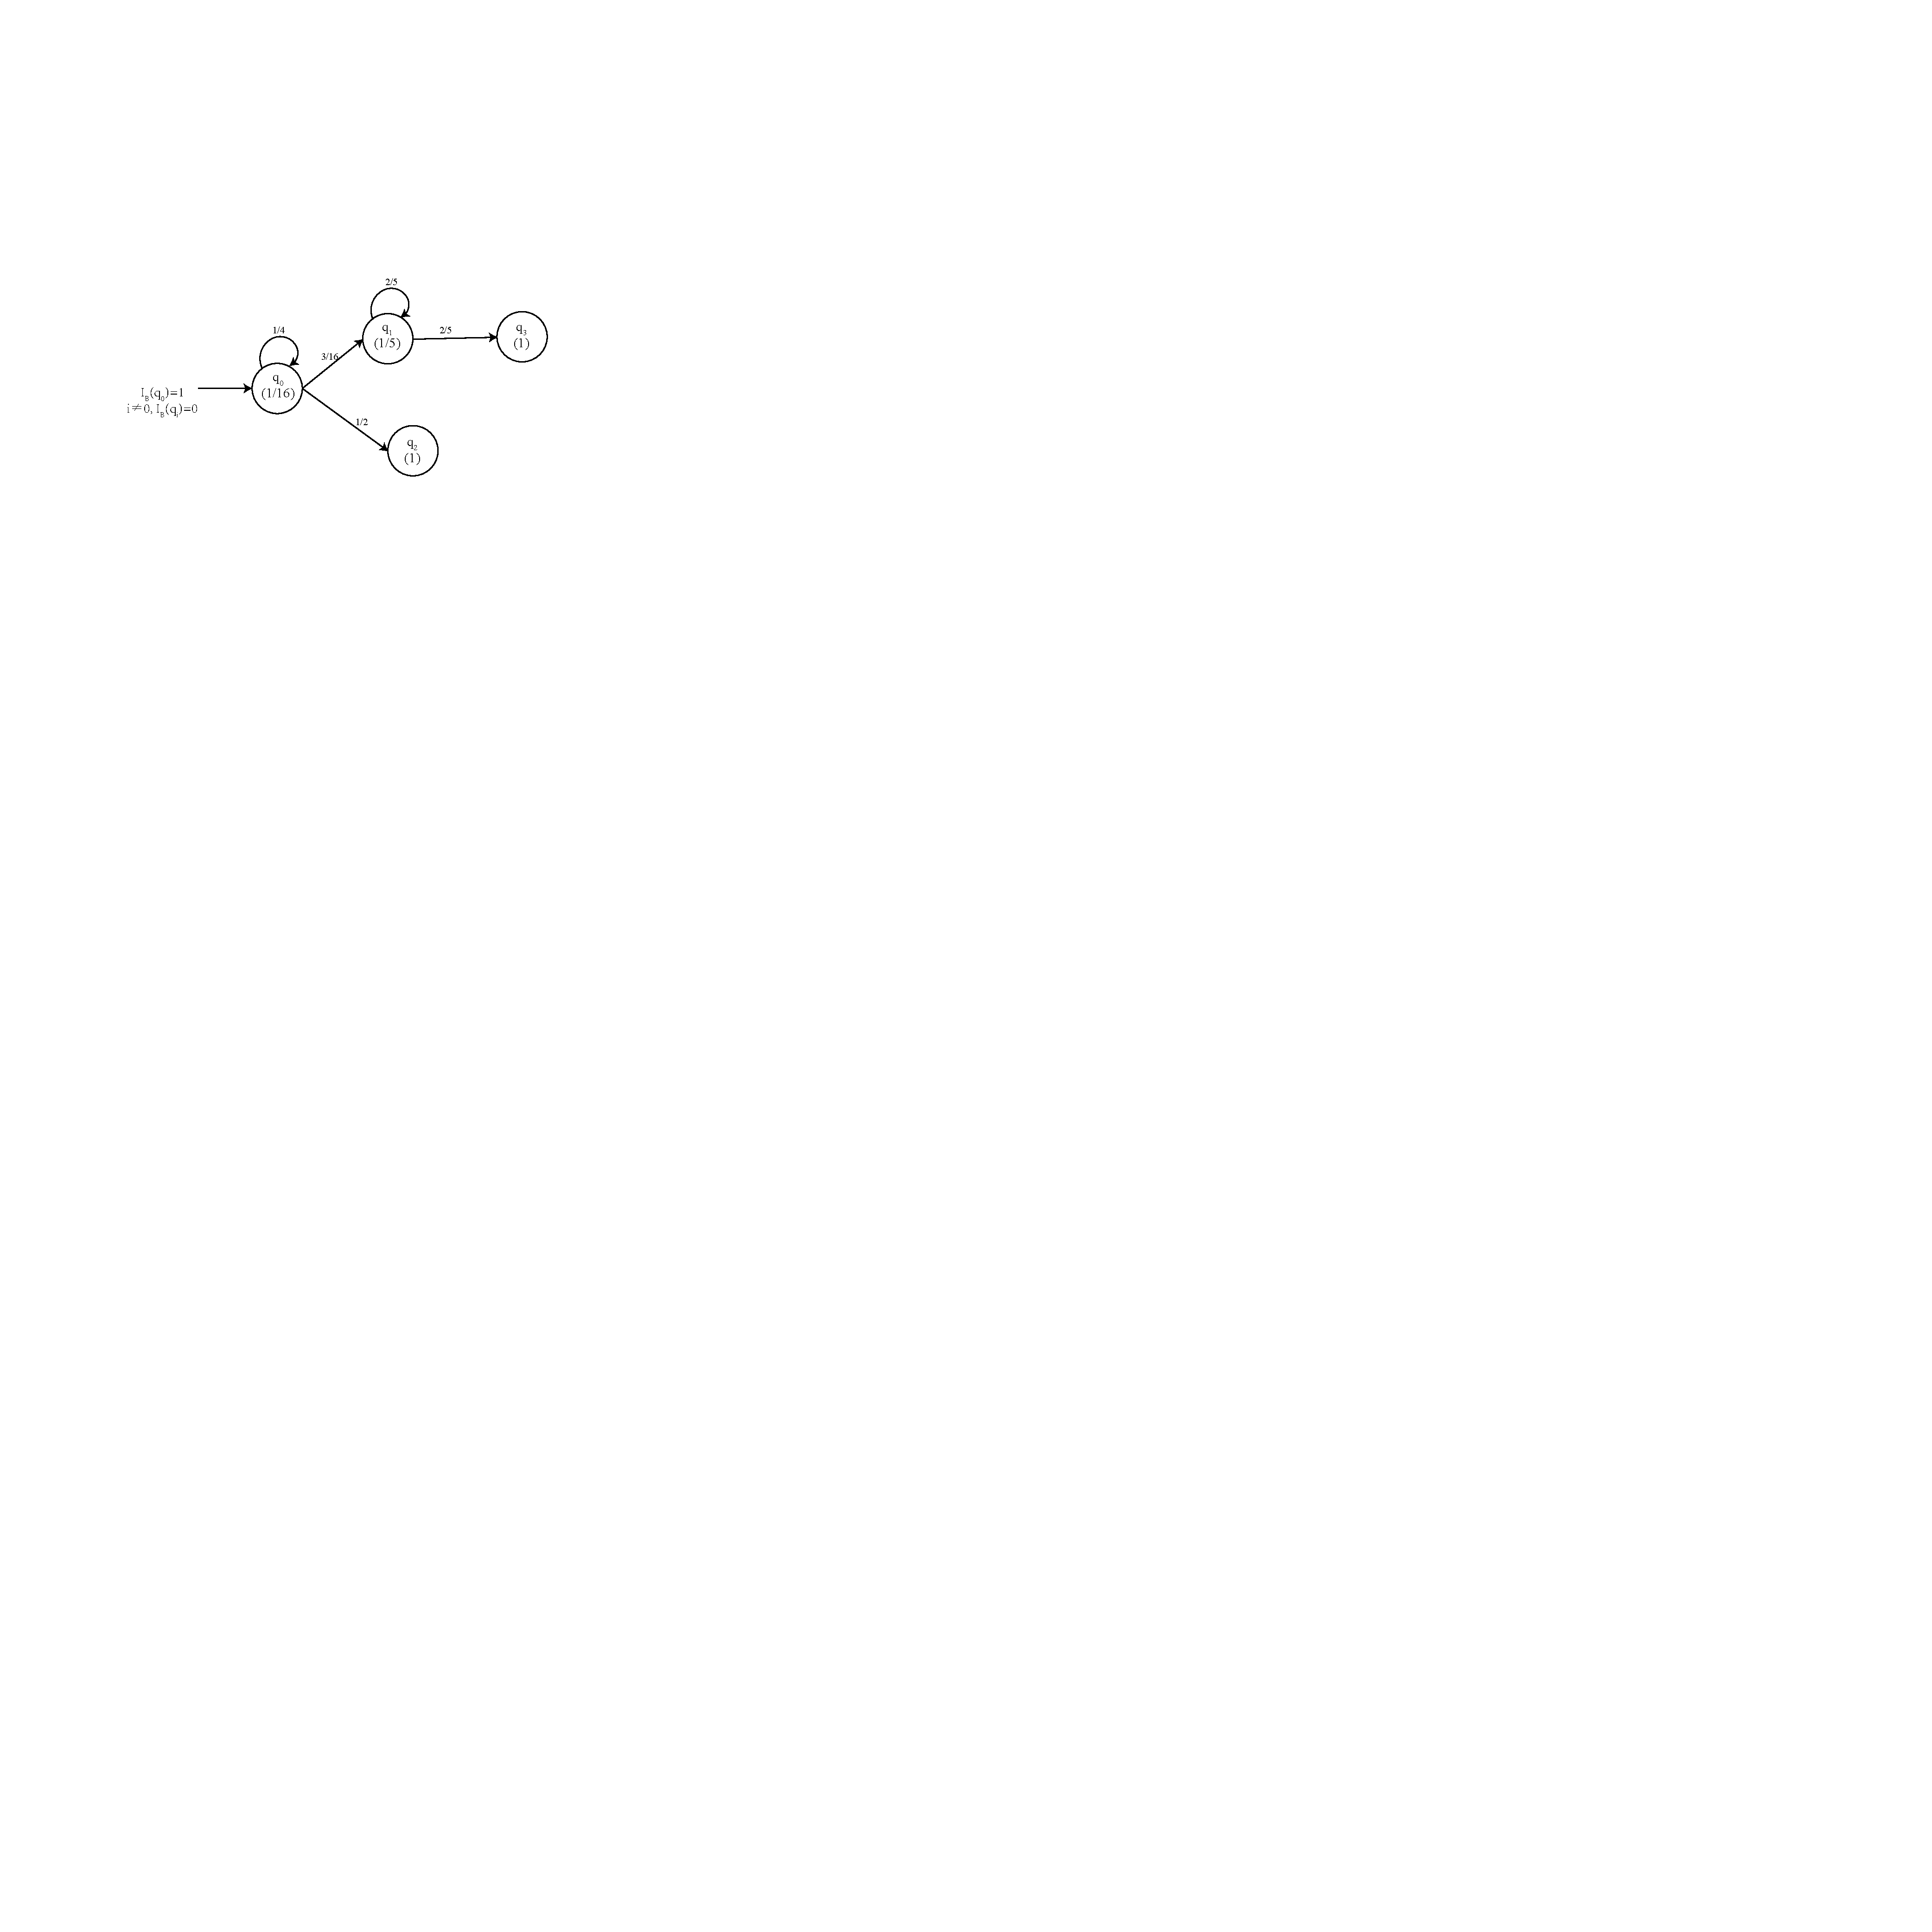
\includegraphics[width=300pt]{PFSA_example.pdf}
                \caption{概率有限状态自动机的可视化表示}
                \label{fig:PFSA_example}
            \end{figure}
            
            概率有限状态自动机是一种随机模型, 它生成的是在有限串集合$\Sigma^{*}$上的概率空间. 对于此自动机, 生成一个串的步骤为:
            
            \begin{itemize}
                \item 初始化: 按照概率分布$I_\mathcal{B}$选择一个$Q_{\mathcal{B}}$中的状态$q_0$作为初始状态;
                
                \item 生成: $q$表示当前状态. 以$F_{\mathcal{B}}(q)$的概率决定是否在此状态处终止, 或者以$P_{\mathcal{B}}(q, a, q')$的概率决定是否进行转移$(q,a,q')$. 如果进行此转移, 则输出$a$并将$q'$置为当前状态.
            \end{itemize}
        
            概率有限状态自动机的以下特点让其适用于使用场景的建模:
            
            \begin{itemize}
                \item 自动机的状态可以很方便地与服务端点关联起来. 因此, 状态的转移可对执行序列进行建模.
                
                \item 自动机的字符集$\Sigma$可建模服务端点的所有可能的响应. 另一方面, 每个状态转移均对应一个字符$c \in \Sigma$, 其表示此转移仅适用于当前读入字符为$c$的情形. 因此, 这个对应字符可建模各个转移所适用的范围, 此范围由服务端点的返回响应决定. 也就是状态转移对应的字符定义了进行此状态转移的条件.
                
                \item 自动机的起始概率, 终止概率, 转移概率反映了进行不同交互的频率差异.
            \end{itemize}
            
            然而, 在使用场景模型中关键的数据约束, 数据依赖, 测试断言则很难在概率有限状态自动机中表达与反映. 本文的场景模型扩展了概率有限状态自动机模型来克服这些问题.
        
        \subsection{模型定义}
            本文的场景模型在以下方面扩展了基本概率有限状态自动机:
            
            \begin{itemize}
                \item 它在状态定义中加入了请求数据约束与请求数据依赖的定义, 以便于生成请求数据.
                
                \item 它在状态定义中加入了响应数据约束与测试断言 的定义, 以便于对响应进行验证.
            \end{itemize}
            
            形式化的定义如下:
            
            \begin{definition}
                \label{def:our}
                场景模型是一个元组
                \begin{equation}
                     \mathcal{A} := <Q_{\mathcal{A}}, \Sigma, \sigma_{\mathcal{A}}, I_{\mathcal{A}}, F_{\mathcal{A}}, P_{\mathcal{A}}>,
                \end{equation}
                
                其中:
                \begin{itemize}
                    \item TODO
                \end{itemize}
            \end{definition}
        
        \subsection{解释与说明}
        
        \subsection{示例}
    
    \section{测试生成方法}
    
    \section{*测试场景优化}

